\section{Word Embedding}
Considering a word, you have to represent it as a vector, it means that exists a multi-dimensional space [the dimension is due to the cardinality  of the vector], 
where you have to represent the word. This space is called \textbf{Embedding} of the word. \\
Word Embedding means finding a space where you can represent words. An embedding is a representation.

Imagine you have a certain experience E, and let's name it $D = x_1, x_2, ..., x_N$, you can describe:
\begin{itemize}
    \item[--] Supervised Learning: given the desired outputs $t_1,t_2,...,t_N$ learn to produce the correct output given a new set of input
    \item[--] Unsupervised learning: exploit regualrities in $D$ to build a representation to be used for reasoning or prediction
    \item[--] Reinforcement learning: [not relevant]
\end{itemize}{}

Word Embedding is Unsupervised learning since it is exactly: exploiting regularities in the text to find a space (an embedding) where you can represent the text in a way it makes you useful for reasoning or prediction.  \\
%You have to take one word and you have to represent it as a vector, it means that exist a multi dimensional space (where the dim is due to the cardinality of the vector). This space where you put the word is called Embedding of the word. 

%Word embedding means finding a space where you can represent words. An embedding is a representation.
 
%recall slide 2 - 3
%slide 2
%Word embedding is Unsupervised learning, word embedding is exactly: exploiting regularities in the text to find a space (an embedding) where you can represent the text in a way it makes you useful for reasoning or prediction. 

Briefly recall on Neural Autoencoder: get an input, project it in a "latent space" (a space where you have a number of dimension to which the input will be compressed ) and then you decompress the input into the original space in such a way that you can reconstruct all the original information.\\
Doing this, you are:
\begin{itemize}
    \item[--] Limiting the number of units in hidden layers (compressed representation)
    \item[--] Constraining the representation to be sparse (sparse representation)
\end{itemize}{}
Neurons in the hidden layer represent categories, so the goal is to push the inner representation to have as many zeros as possible (you want that your input belongs to a class or few classes). \\
This model has an additional constrain that allow to \textit{sparsify} this representation. \\
This kind of model start from a space which 
$$
\begin{array}{c}
{x \in \mathfrak{R}^{I} \stackrel{\text { enc }}{\longrightarrow} h \in \mathfrak{R}^{J} \stackrel{\text {dec}}{\longrightarrow} g \in \mathfrak{R}^{I}} \\
{I >> J}
\end{array}
$$
After the decompression, the goal is to have $x$ and $g$ as similar as possible. This is allowed by the minimization of an error function which is 
$$
E=\underbrace{\left\|g_{i}\left(x_{i} | w\right)-x_{i}\right\|^{2}}_{Reconstruction Error}+\underbrace{\lambda \sum_{j}\left|h_{j}\left(\sum_{i} w_{j i}^{(1)} x_{i}\right)\right|}_{Sparsity Term}
$$
The first term is the squared error of the reconstructed signal $g(h(x)) - x$; the second is the term that enhance the sparsity.
%slide 3
%Neural Autoencoder: you have an input, you project the input in a "latent space": a space where you have a number of dimension where your image will be compressed and then you decompress the image into the original space. You can think about Neural Autoencoder as a model which takes an input, it compress it in a latent space (reduced space) in such a wa yyou can reconstruct all the information that are originally contained in the data. 

%The original use of NAutoencoder was clustering where each of these nodes were one on the cluster the input belongs to. So the idea is that you limit the number, creating a sort of bottleneck (la parte in mezzo tra encoding e decoding), you push through this bottleneck all the input, you reconstruct the input as output of this model the original input. To obtain the result, you have to push this inner representation to have as much as possible zeros. I neuroni nel bottleneck rappresentano ciascuno categorie diverse.

%Sometimes this model has an additional constrain that allow to sparsify this representation: means that the vector of output in the middle layer has a lot of zero, it is characterize by few values different from zero. To do it, you want that an input after encoding and decoding to be equal to the original one. This kind of model start from a space which 
%$$
%\begin{array}{c}
%{x \in \mathfrak{R}^{l} \stackrel{\text { enc }}{\longrightarrow} h \in %\mathfrak{R}^{\prime} \stackrel{\text {dec}}{\rightarrow} g \in %\mathfrak{R}^{\prime}} \\
%{I >> J}
%\end{array}
%$$

%At the end you want that after the decompression, x and g are as similar as possible. This is obtaining by minimize an error function which is the squared error of the reconstructed signal g(h(x)) - x [the original], and usually you add a term which tries to sparsify the output: I want the absolute value of $h_j$ so the output of the middle neurons to be as equal as possible to zero. You use absolute value because if you use a square you push the output to zero but in a sort of uniform way, so you get the output small but no one will be equal to zero. While if you use abs you minimize the overall sum by putting as much as possible of them to zero (l1 normalization, lasso). 

Natural Language processing treats words as discrete atomic symbols: among the list of all possible objects, the term 'cat' is an id. So words are basically id symbols for objects, and a language is a set of symbols and rules to combine them. \\
In this way, a sentence is a set of words  with very high sparse representation. \\
One of the typical representation of  text is the \textit{Bag-of-Words} representation: take text, represent it with a vector with 1 in the first position if first word in the bag is in your text, 0 otherwise. \\
If the possible words are $N$, the space is $2^N$ since for each word you can have 1 or 0 (there is or nor). The problem is that when you represent text, you will end up with an huge representation which is impossible to explore with data. \\
Most of the time you divide your vector by the frequency of which the corresponding word appears. So you perform something like TF-IDF: discounts the occurrences by how frequent a term is. \\

The results is a sparse and high-dimensional vector $\rightarrow$ Curse of Dimensionality:\\ 
exponential complexity in terms of data that you need to estimate a multi-dimensional distribution. The more is the space and the more sparse it is, the more becomes impossible to learn a distribution.


%slide 4
%Let's talk about text, which is made by words: words are symbols which represent context. If you think about the list of possible object, the term cat has an id. Word are basically id symbols for objects. Language is a set of symbols and rules to combine these symbols. A word is an item in a dictionary. If you think to a sentence as a set of words is a very sparse representation. One of the typical representation of the text is the Bag-of-Words representation: you take text, you represent with a vector which say 1 in the first position if you have the first word in your text, 0 otherwise. 
%if you have 32 possible words, your space is $2^32$ since for each word you can have 1 or 0 (there is or nor). The problem is that when you represent text, you end up with an huge representation and it is impossible to explore with data.
%Most of the time you divide your vector by the frequency of which the corresponding word appears. 
%So you do an encoding like TF-IDF: discounts the occurrences by how frequent a term is. 

%So you have a sparse vector and what happen is that text is sparse in high dimension, Curse of Dimensionality: exponential complexity in terms of data that you need to estimate a multi dimensional distribution. The more is the space and the more sparse it is, the more becomes impossible to learn a distribution.

%slide 5
\subsection{Encoding Text}
%How you encode text?
Performance of real-world applications depends on input encoding. There are two main approach to encode text: \textit{Local representation} and \textit{Continuous representation}. \\
In Local representation, you look to each word by looking around it. 
\begin{itemize}
    \item \textit{Bag-of-Words}: represent a document like a N-dimensional vector, where N is equal to the number of words in your dictionary (bag). The vector contains 1 in the first position if first word in the bag is in your text, 0 otherwise. The same for each position. 
    \item \textit{N-grams}: it represents a word probability by a probability distribution which is based on the previous N-1 terms. 
    \item \textit{1-of-N coding}: it not represent the text but a word. It becomes unfeasible to perform some relevant representation of the text
\end{itemize}{}

%Bag of word: you represent a document like a vector where the number of word that appear in the document has a reprentation of the qualcosa

%N-grams: it represents a word probability by a probability distribution which is based on the previous two N-1 terms. 

%1-of-N coding: it not represent the text but a word. cat = id537 is represented as a set of zeros and one 1 on the position 537. Then with this single words you can create a text by justappose all these vectors. It becomes unfeasible to perform some relevant representation of the text.

%The previous are local representations: you look each word by looking around it.

In Continuous representation, you use some probability distribution to encode the text:
\begin{itemize}
    \item \textit{Latent Semantic Analysis}
    \item \textit{Latent Dirichlet Allocation}
    \item \textit{Distributed Representations}
\end{itemize}{}


%Another kind of representation are the continuous representations: they uses some probability distribution. This continuous distribution is based on the topic or on the language. 
%We will only see N-grams because word embedding started from this. 

\subsubsection{N-grams}
The idea is that you describe the way you write a text by a probability distribution in such a way that if you want to understand what is the probability of a given document, you have to compute the join probability of observing word 1 in position 1, word 2 in position 2 and so on. \\
So you take a word and, basing on it, you take another bag-of-words where the probabilities are different and they depend on the word extracted. It is complex because you need as many bags as the possible word to be extracted. \\
For Bag-of-word you need only one bag. Too simple \\
For N-grams, when N=1, you only need the previous word, so a bag for each word you might extract. In N-grans, in general, you need $N^N$ bags each time. \\

To be more precise, define a N-grams in a Language Model means: \\
Determine $P(s=w_1,..,w_k)$ in some domain of interest
$$
P\left(s_{k}\right)=\prod_{i}^{k} P\left(w_{i} | w_{1}, \dots, w_{i-1}\right)
$$
means that in order to predict the probability of a word in a sentence, you can multiply the probability of each word given the previous ones. 
In traditional N-grams language models "the probability of a word depends only on the context of $n-1$ previous words"
$$
\widehat{P}\left(s_{k}\right)=\prod_{i}^{k} P\left(w_{i} | w_{i-n+1}, \dots, w_{i-1}\right)
$$
The space is very sparse and the amount of text you have, do not cover it entirely, so you might have a lot of zeros. It might happen that you have never seen a word after another, in particular in the text you are considering. Because of this sometimes you have a smoothing procedure which basically adds one occurrences to every possible combination, so no zero anymore. \\
Typical ML-smoothing learning process (e.g. Katz 1987), where first compute \\
$
\widehat{P}\left(w_{i} | w_{i-n+1}, \dots, w_{i-1}\right)=\frac{\# w_{i-n+1}, \dots, w_{i-1}, w_{i}}{\# w_{i-n+1}, \dots, w_{i-1}}
$
and then smooth to avoid zero probabilities. \\
%slide 6
%N-grams is a way to describe a language. 
%The way you write text: start from the first term and based on that, the next term has not a uniform probability. You describe the way you write a text by a probability distribution, so that if you want to understand what is the prob of a given document, you have to compute the join probability of observing word 1 in pos 1, word 2 in position 2 and so on. 

%In bag of word, you model this as independent sampling with replacement, it is the simplest one. 

%In a more modern languages, you describe the prob of each word as dependent by the previous term. You can push even forward: you can look at the word written before and the one you will write. [quasi inutile scriverlo]

%What we do is that we pull out a word and basing on that word we take another bag of words, where the prob. are different and depend on the word just extracted and repeat the process. Complex because I need as many bags as the possible words to be extracted.

%So for bag of Words I need one bag.
%For N-grams, where N is 1 gram, you only need the previous word, so you need a bag for each word you might extract. In N-grams in general, you need $N^N$ bags to extract everytime.

%The idea is that Bag of words is too simple. 

%So far we talk about how represent a text, now we shift in how a text is generated. 

%slide 5 [quadratino con le prob. ]
%We assume that our language model is given this way to predict the prob. of a sentence, you can multiply the prob. of each word given the previous ones. 
%[Prima formulina]
%You can compute that by the conditional prob. of one word given the others: you simply look in the text how many times w1 appears when there is this sequence of words and how many times w1 does not appear. The space is very sparse, the amount of text you have is not covering it, you might have a lot of zeros: it might happen that you have never seen a word after another, in particular in the text where we are looking in it has never seen. Because of this sometimes you have a smoothing-procedure which basically adds one occurrences to every possible combination, so you will not have zero anymore. 

%slide 6
The problem with this approach is that N cannot be too big, the curse of dimensionality depends on N. \\
Let's assume a 10-gram Language Model on a corpus of 100.00 unique words. 
\begin{itemize}
    \item[--] The model lives in a 10D hyper-cube where each dimension has 100.000 slots
    \item[--] Model training $\rightarrow$ assigning a probability to each of the $100.000^{10}$ slots: for each possible combination of 10-words before, compute the probabilities of my 100.000 words.
    \item[--] \textit{Probability mass vanishes} $\rightarrow$ more data is needed to fill the huge space:
    \item[--] A solution can be to add more data, but it increases number of unique words! $\rightarrow$ Is not going to work!
\end{itemize}{}
In practice, corpuses can have $10^6$ unique words, but the contexts are typicaaly limited to size 2 (so 3-gram model). It means that the correlations between words represented in this language model are very short and a lot of information is not captured. \\

%This 10-gram language model leads to a 10 dimensional hypercube. For each possible combination of 10 words before, you have  to tell me what is the probability of my 100000 words. You see that you need, for training, to assign a prob. to each of the 100.000 of words. 
%The problem is that to fill this, you need to have a lot of data, to hundred times the number of slots in order to have good accuracy. At least ten times the number of slots. Because this, you end up not be able to estimate these probabilities. A solution is adding more text, but the more text you have, the more unique words you get, not a good idea. 

%In practice:
%Basically what happens no one so far has been able to push this model more than 3 grams. It means that the correlation between words represented in this language model are very short: you can have only very short correlated text. 

Suppose we observe the following similar sentences:
\begin{itemize}
    \item \textit{Obama speaks to the media in Illinois}
    \item \textit{The President addresses the press in Chicago}
\end{itemize}{}
With classical one-hot-encoding vector vector space representation, we have:
\begin{itemize}
    \item[--] speaks = [0 0 1 0 .. 0 0 0 0]
    \item[--] addresses = [0 0 0 0 .. 0 0 1 0]
    \item[--] obama = [0 0 0 0 .. 0 1 0 0]
    \item[--] president = [0 0 0 1 .. 0 0 0 0]
    \item[--] illinois = [1 0 0 0.. 0 0 0 0]
    \item[--] chicago = [0 1 0 0 .. 0 0 0 0]
\end{itemize}{}
This approach is already unfeasible at computation, furthermore in this way you cannot state when two sentences means the same thing: 'speaks' and 'addresses' are referenced as two different words and the corresponding vectors are orthogonal. The same for each vector. So this model ignores synonyms or other form of symmetries $\Rightarrow$ \textbf{Word Similarity Ignorance}: word pairs share no similarity (don't take into account semantics) and we need word similarity to generalize.\\

%slide 7
%The problem is: if we use this approach which is already unfeasible at computation prospective, you will never ever say that those two sentences means the same thing. This because speaks and addresses will be represented as different words and the corresponding vector are orthogonal, the same for the other vector. So not only the sequences of terms can be only short, but this model, where you try to represent word as an index in a vocabulary, ignores sinonimous or other form of symmetries in the text.
%You seen that what was done until the 90's was working, but have significant issue related to short time correspondences and very sparse representation which is not taking into account semantics.

\subsubsection{Embedding}
\textbf{Word Embedding} is a technique to map a word (or phrase) from it's original high‐dimensional input space (the body of all words) to a lower‐dimensional numerical vector space ‐ so one embeds the word in a different space. \\ 

You start from a long sentence and you want to project it in a lower dimensional space in such a way that this sentence, when you try to reconstruct it, has the same meaning. The idea is that terms with a close semantic are mapped close each other in the lower-dimensional space: closer point are closer in the meaning and they form clusters. \\
By forcing term with similar meaning to stay close, you have a compression which maintains also the meaning. \\

%slide 8
%The idea of word embedding is to find a representation from high dimensional space into a lower dimensionality space (this is the idea of embedding, it is like the idea of the encoder): you start from long sentence, you want to project it in lower dimensional space in such a way that this sentence when you try to reconstruct has the same mean. 
%The idea is that you take these terms and you map them one to one in lower dim space where you would like to have close point in the space having close semantics (meaning). You would like to compress in such a way that two words that have the same semantics are close. It means that if you make an error in decompressing and you change a term for another, it is not a problem because you  preserve the semantic of the sentence. So instead of having a huge bit streams (come nella slide precedente), you want to have one point in the space. What should happen is that by forcing terms with similar meaning to stay close, you have a compression which has also some meaning.

How to do it? \\
Each unique word $\boldsymbol{w}$ in a vocabulary $V$ (typically $|V| > 10^6$) is mapped to a continuous $m$-dimensional space (typically $100 < m < 500$): 
$$
w \in V \quad \stackrel{\text { mapping } C}{\longrightarrow} \quad \mathfrak{R}^{m}
$$
The trick is that you move from a very sparse boolean space in a continuous real-valued space: in the latter you have a lot of space w.r.t. binary one since instead of having only 1 or 0, you can specify a real value. \\
The goal is to finding a mapping from the original space into a real-valued space. \\
In this way we are fighting the Curse of Dimensionality with:
\begin{itemize}
    \item[--] Compression (\textit{dimensionality reduction}): similar words should end up to be close to each other in the feature space. 
    \item Smoothing (\textit{discrete to continuous}): if you don't have a word in a particular point, you just need to go close that point to find words with same meaning
    \item Densification (\textit{sparse to dense})
\end{itemize}{}

%slide 9
%How to do it?
%Take a word w in a vocabulary, which is $10^6$ dimension, and you map it in a continuous space which has a number of dimensions lower than the original one. You want to start in high dimensional space like $10^6$ and you want to project this representaition into a lower continuous representation with lower dimension.
%The trick and the effectiveness is that you move from a very sparse boolean space in a continuous real value space. So in a real space you have a lot of more space wrt binary space, in fact between two real value, ce ne può essere un altro, quindi si possono rappresentare molte più cose con meno dimensioni, poiché abbiamo molti più valori diversi tra loro da poter utilizzare. 
%The idea is to finding a mapping from the original to the real valued space. The results is the position in the space of the obama word. 

%We have the effect of compression, we have smoothing because if  you do not have a word in that point, you can go closest point (you have a sort of geometrical smoothing in this space); you have densification which comes from dimensionality reduction and smoothing effect. 

One idea to go beyond the Katz model is proposed by Bengio: he used a Neural Autoencoder to build a non-linear continuous language model. \\
He tried to predict what would be the next word, representing the language model (the prob. of the next word given the previous one) as a classification problem. \\

\begin{minipage}{\linewidth}
        \centering
        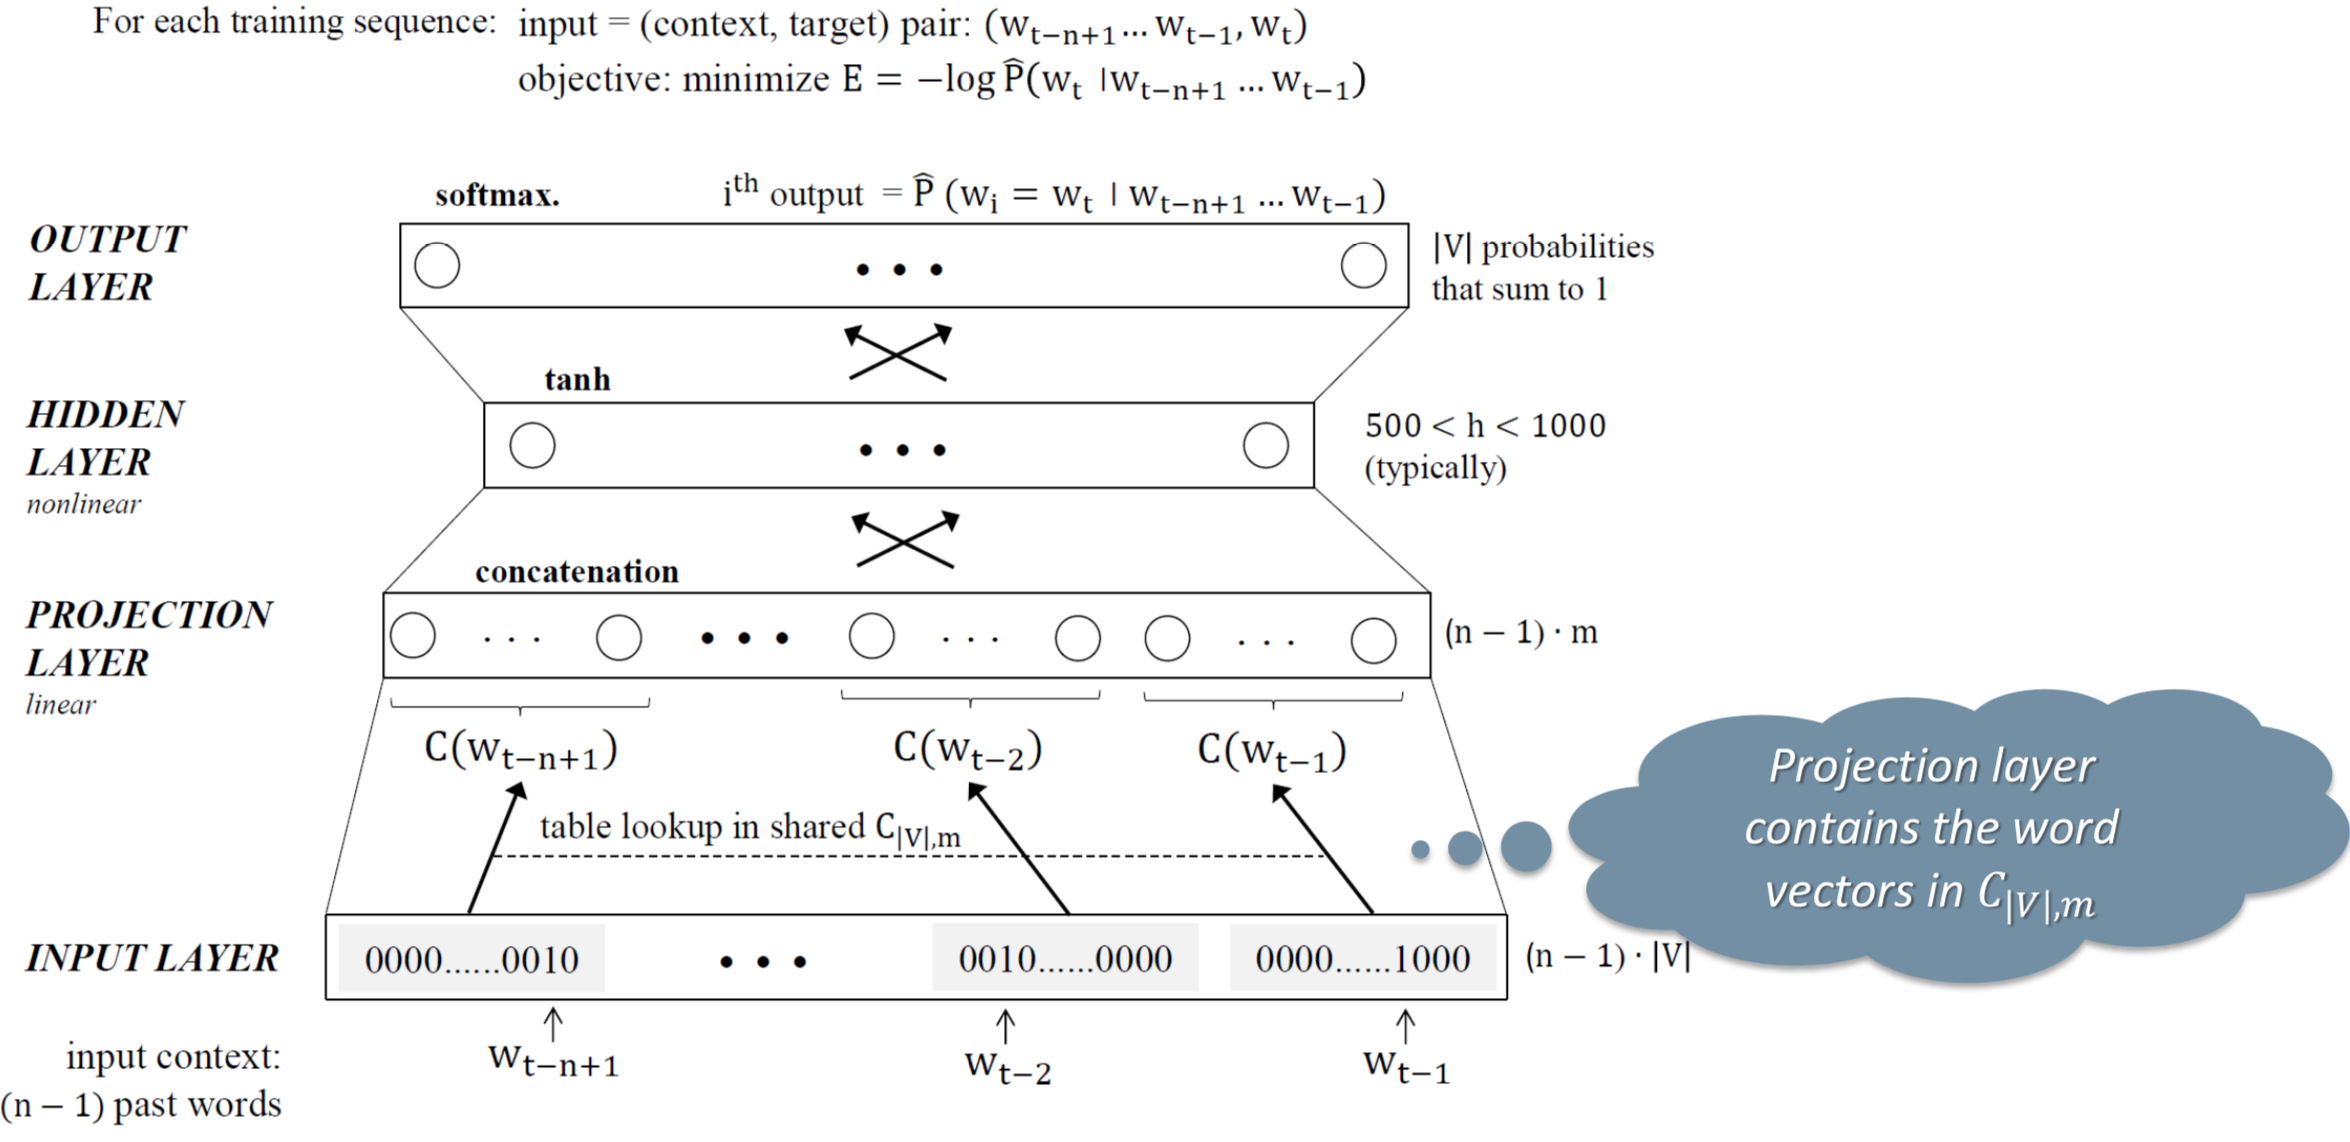
\includegraphics[width=15cm, height=6.5cm]{images/an_embedding.png}
        %\captionof{figure}{The model pipeline.}
        %\label{fig:flow_fig}
\end{minipage} \\

The inputs are a $(n-1)$ vectors of size $|V|$ in one-hot-encoding representing past words. You project each vector in a subspace, concatenate these projections and get the predictions by a softmax, trying to predict which word will be the next one. It's not exactly an autoencoder but the idea is to start from an high dimensional space, compress and decompress. It's not symmetric. \\
It tries to minimize the cross-entropy between the output of the network and the observed class: 
$$
min \mathrm{E}=-\log \widehat{\mathrm{P}}\left(\mathrm{w}_{\mathrm{t}} | \mathrm{w}_{\mathrm{t}-\mathrm{n}+1} \ldots \mathrm{w}_{\mathrm{t}-1}\right)
$$
%slide 10
%How to do that?
%One idea to go beyond the Katz model is proposed by Bengio. The idea is to use a neural autoencoder to build a non linear continuous language model. 
%They are trying to predict what would be the next word, trying to represent the language model (the prob of the next word given the previous one) as a classification problem. 
%You have this one-hot-encoding, so n-1 vectors of V size, where V is the number of words in the vocabulary. They are projecting them in a subspace then concatenate these projections and then with a neural network and a softmax layer they try to predict which would be the next word. They try to implement language model with the neural network. They take the word, they build a continuous representation of this word, then they compress this continuous representation into an hidden layer of 5 hundred real values and based on this they try to predict what's the next word. 
%It's not exactly an autoencoder, but the idea is to start from an high dimensional space, compress and decompress it. It's not symmetric. 
%You train as a classification model. 
%You want to minimize wrt the cross entropy between the output of the network and the observed class [è scritta sopra la figura].

\begin{wrapfigure}{l}{6cm}
    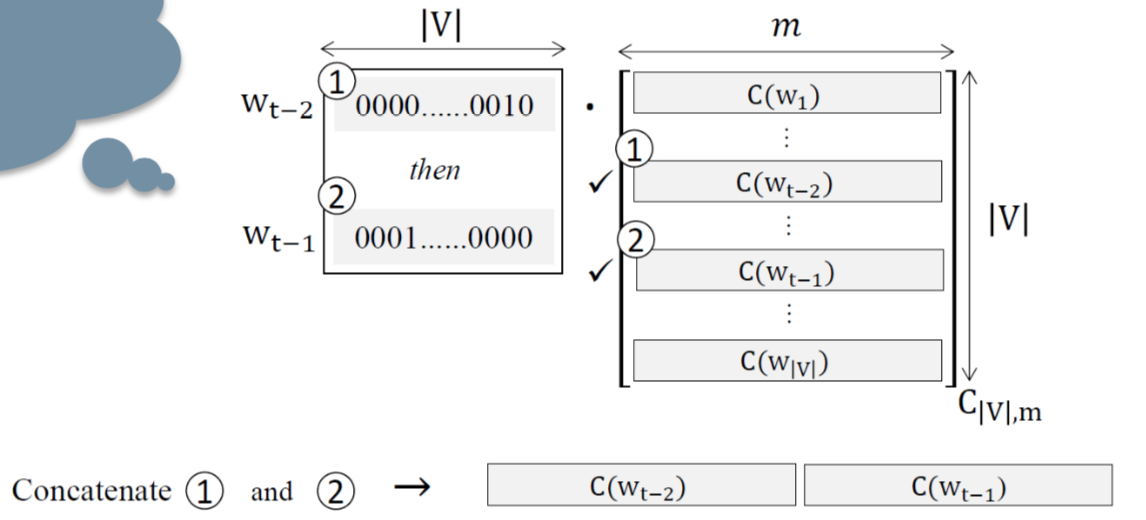
\includegraphics[width=6cm, height=3cm]{images/emb_matrix.png}
    %\label{fig:lstm_org}
\end{wrapfigure}  

The interesting part is to take the word and project to a smaller representation of size $m$: to do this, you learn a matrix that takes the word and it compresses it. \\
This matrix has $m*|V|$ elements and these are the parameters of your model: this matrix compress the one-hot-encoding representation into an m-dimensional representation. [This matrix is the 'trick']\\ 

If you have two words (in ohe) of time $t-1$ and $t-2$, you compress them one by one using the matrix, and then concatenate the results. \\ 
%slide 11
%[la matrice di cui si parla è quella nella figurina di grandezza m*V]
%The interesting part is to take the word and project to a smaller representation of size m: to do this, you learn a matrix that takes the word and it compresses it in a smaller representation. 
%This matrix has m*V elements and these are the parameter of your model and this matrix are compressing the one-hot-encoding representation into an m-dimensional representation: this matrix is doing the trick.
%Then you concatenate the two word, then compress them, classify and you get the new word. 

%slide 12
%Usually what you get is a softmax output. The input of the softmax is the tanh of this hidden layer, the hidden layer is obtained by a mixing matrix. 
%1:00:00 descrizione encoder
%Inserire modello pag 11

The brilliant idea of this model is this sharing of weights (the matrix $m*|V|$), because doing the FC explodes in terms of weights. \\
The training of this network by stochastic gradient descend has a \textit{complexity} of \\
$m*V$ (the matrix) + $n*m*h$ (it is the FC) + $h * |V|$ (the softmax). \\ \\

%slide 13
Once you have trained by SGD, they (Bengio et al.) tested the model which improves the performance of 24\% the state of the art. \\
The problem is that it is unfeasible to use it on large corpus because of the complexity in training, at least in time. So it is not work perfectly overall. \
The interest part is that Bengio and colleagues were aiming at beating this benchmark and they didn't recognize that they invented Word2Vec.

\subsubsection{Word2Vec}
The idea is: achieve better performance allowing a simpler (shallower) model to be trained on much larger amounts of data 
\begin{itemize}
    \item No hidden layer (leads to 1000X speed up)
    \item Projection layer is shared (not just the weights matrix)
    \item Context contains words both from history and future
\end{itemize}{}
The goal of Word2Vec is to overcome the issue in complexity by removing as much parameters as possible and keeps only the relevant ones: the relevant ones are those of the projection from a sparse space in a dense space. \\
So Word2Vec removed the hidden layer, shared the projection layer and add both word from the history and from the future to predict the missing one. \\

The main idea comes from the following quote:
\begin{quote}
    \textit{"You shall know a word by the company it keeps"} ,  John R. Firth, 1957:11.
\end{quote}{}
which means that the model tries to understand a word by the the words next to it. \\
The meaning of a word is given by the distribution of the word around it. If one word has same words next to it as another word, probably the two words are the same thing. You just need to project the neighbouring word into the same place and you are able to identify similar words.  
%slide 14
%Others autors recognize the work of Bengio as word2vec because the matrix that takes a vector of size V and project into a vector of size m is doing what the Embedding idea was doing: taking a sparse vector, project it in a lower dimensional real valued representation, and this representation was good because with it you could predict what would be the next word, so were not loosing the information in this set of vector. 
%Basically the idea is to use this model (bengio) in order to learn what is the best representation for each single word in the vocabulary so that a language model build on that was able to fit language distribution.
%So Mikolov says, since the most issue is in complexity, let's remove as much as possible parameters from the model and keep the relevant ones: they realize that the relevant one were those projecting from the sparse to the dense space, if you do this job, things would be easy later on. 

%The idea of word2vec is that they remove the hidden layer; if my encoding is good, I should be able to perform good without the hidden layer; Also the projection layer to be shared and to add both words from the history and the future to predict the missing word. 

%Make an example: assume you read this text and use all these words to represent and predict this one (non so quale). The idea is that you try to understand a word by the words next to it; if you are able to represent Neymar by the weight these other words project, then basically this representation is equivalent to the word. 
%The meaning of a word is given by the distribution of the word around it. If one word has same words next to it as another word, probably the two words are the same thing. 
%I just need to project the neighbouring word into the same place and I basically project two words in the same point.  
%It is literally a lookup table. 

%slide 15 (manca la parte principale)
There are two architecture to simplify the Bengio model
\begin{enumerate}
    \item \textit{Skip-grams}
    \item \textit{Continuous Bag-of-Words}
\end{enumerate}{}

%There are two ways of simplifying this complex model (penso quello di Bengio):
%Skip-gram: assume you  have a word, you look for an encoding such that from this enconding you can reconstruct the neighbouring words

%slide 16
%Continuous Bag of word: transform bag of word representation in a bag of words. You have ohe version of this and then you project it into a vector and then predict the ohe of a word. This part is essentially (this part) + directly the softmax. You have a one to one mapping between this word and this vector. You can train it with only text and you try to learn a matrix such that once you project it here, it predicts this word. 

\begin{minipage}{\linewidth}
        \centering
        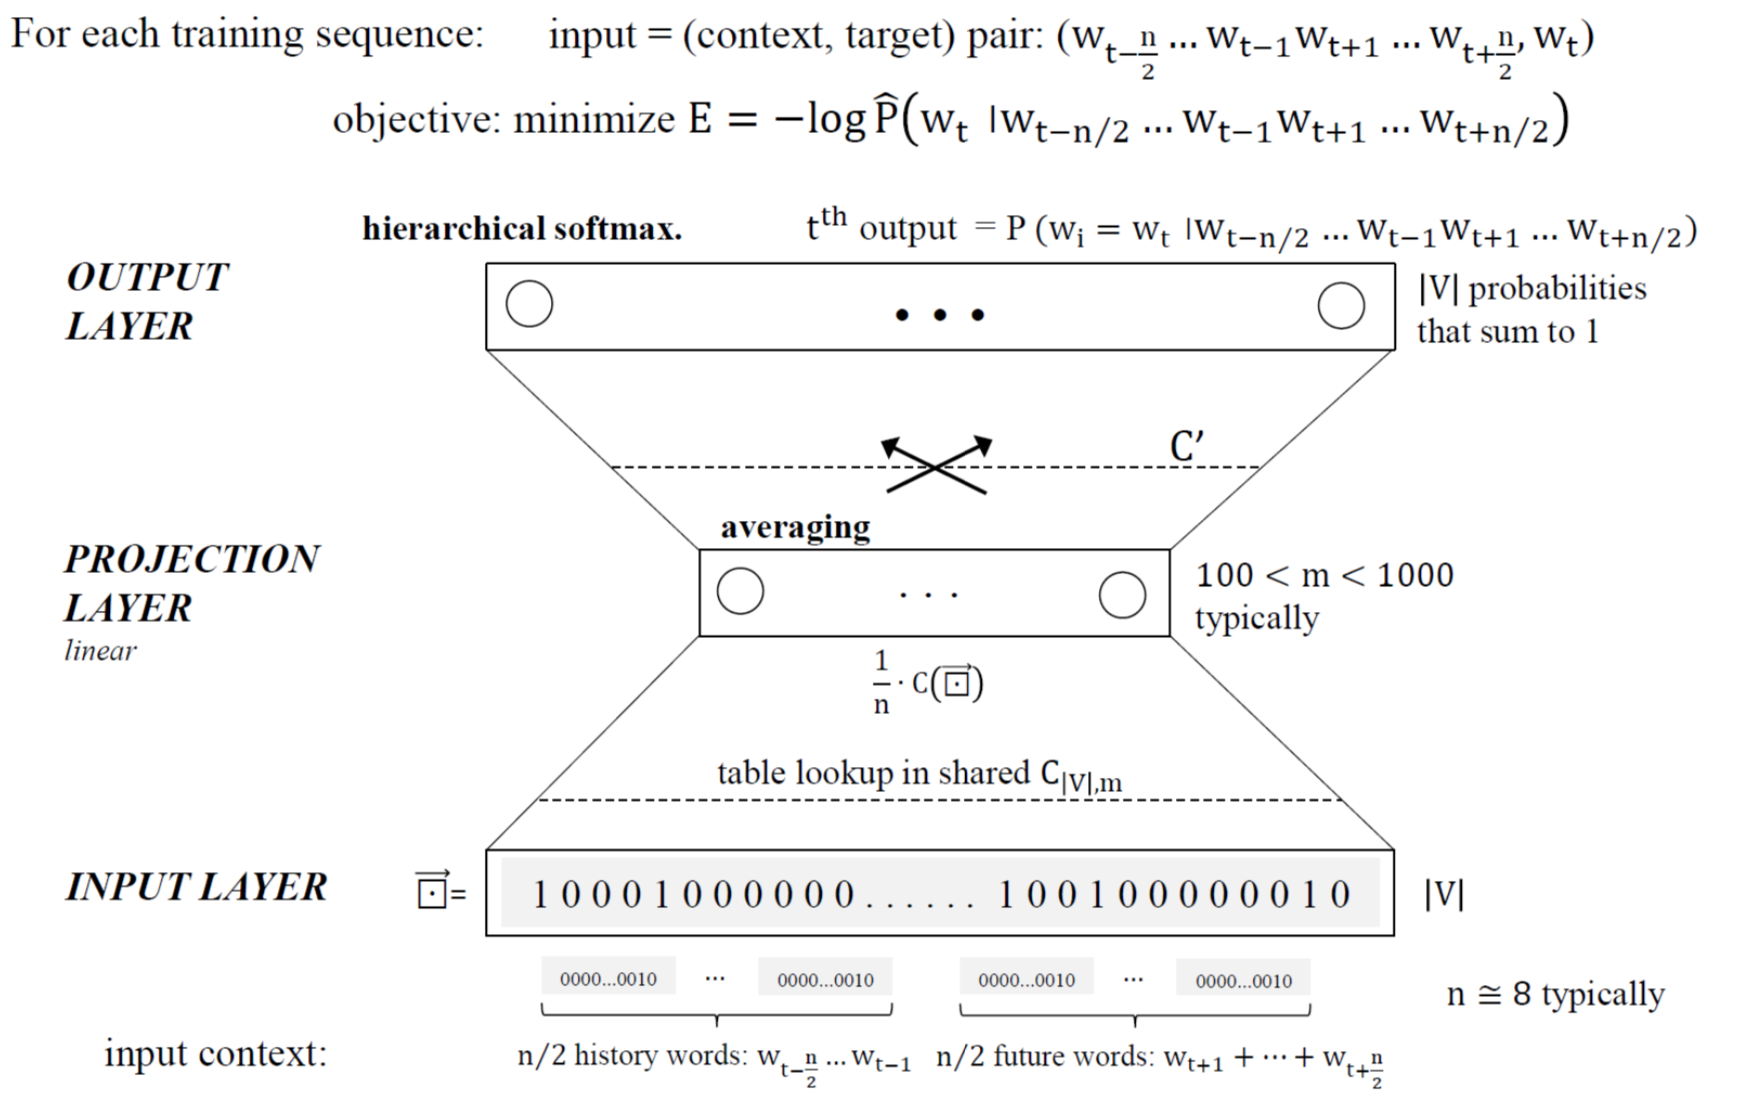
\includegraphics[width=12cm, height=6.5cm]{images/w2v.png}
        %\captionof{figure}{The model pipeline.}
        %\label{fig:flow_fig}
\end{minipage} \\

Procedure: binary encoding, table lookup shared among n words, instead of concatenation you will use averaging because it is smaller in a way that the result is $m$, not $m * n$ (? not sure about that). From this average you predict one of the words. \\
%slide 18 
The complexity is $n * m +log |V|$: you do not need all the vocabulary but only $log |V|$.\\
This model somehow is able to learn language model, but you are much more interested in how to learn an embedding of each word in such a way it represents the structure in the language model in this real valued space. \\

%This model somehow is able to learn language model (in the sense that I give you n words and I give you what is the prob of the one in the middle giving the others) but you are much more interested in how to learn an embedding of each word in such a way it represents the structure in the language model in this real valued space. With this vector I don't try to predict the word, it represent the word: the way it represents the word is by looking the encoding of the word that happens around it. The point in the space represents the context around this word, the semantic is preserved because two words with the same context are mapped in the same point. 

%slide 19 
%This is why country and capital are mapped near each other and the country-capital distance is more or less the same. You have a sort of constant country-capital difference vector. 

%slide 21
There is some structure in the embedding space where you are projecting the terms and this structure comes from regularities in the text that you want to preserve when you learn a language model. \\
This structure is somehow a sort of algebraic space where you can do operation. Since you have a vector and you assume that vectors have semantic meanings, the idea is that you can do vector operations. \\
What is surprising is that this language tries to structure the space according to regularities and tries to preserve them.  

%slide 25
\subsubsection{GloVe}
The meaning of offset vector in embedding space was emerging from the structure of the language. So the idea of GloVe was to try to predict the ratio between co-occurence probabilities: you do not try to predict the word, you try to predict the ratio between the prob. of k following a word wrt k following another word. You are trying to normalize the vector in the embedding space. At the end, you have to find a meaningful matrix to learn the language. \\

%you do not try to predict the word, you try to predict the ratio between the prob. of k following ice wrt k following steam. You are trying to normalize the vector in the embedding space. At the end you have to find a meaningful matrix to learn the language. 
To Word2vec was word given the context, here they try to model directly ratio between co-occurence, so the ratio between one word appearing when there is one or when there is the other. They minimize a more complex term,
a weigthed least squares. \\
%(la formula non l'ha praticamente spiegata). 
GloVe turns out to be more robust and effective because it tries to enforce what word2vec tries to obtain by chance. \\
GloVe makes explicit what word2vec does implicitly:
\begin{itemize}
    \item Encodes meaning as vector offsets in an embedding space
    \item Meaning is encoded by ratios of co-occurrece probabilities
\end{itemize}{}